\documentclass[10pt]{article}
\usepackage[letterpaper,margin=1in]{geometry}
\usepackage[T1]{fontenc}
\usepackage{lmodern}
\usepackage{microtype}
\usepackage{amsmath,amssymb}
\usepackage{graphicx}
\usepackage{booktabs}
\usepackage{xcolor}
\usepackage[font=small,labelfont=bf,skip=4pt]{caption}
\usepackage[numbers,sort&compress]{natbib}
\usepackage[colorlinks=true,linkcolor=blue!50!black,citecolor=blue!50!black,urlcolor=blue!50!black]{hyperref}
\setlength{\bibsep}{1pt}
\renewcommand{\arraystretch}{0.95}

\newcommand{\Ex}{\mathbb{E}}
\newcommand{\pp}{\,\text{pp}}

\title{\vspace{-1.5em}Optimizing Cloud Virtual Machine CPU Reservations via Optimal Policy Trees}
\author{Chris Low \and Emma Li\\[1pt] \small MIT 15.095 Machine Learning under a Modern Optimization Lens, Fall 2026}
\date{\small December 1, 2026}

\begin{document}
\maketitle
\vspace{-1.8em}

\begin{abstract}
\noindent When a virtual machine (VM) is created, a cloud provider must decide how much physical CPU capacity to set aside before the workload is known. We study it on 2.47 million VMs from the Azure Public Dataset V2 as a prescriptive problem: each VM receives one of four reservation tiers at a modeled cost that charges for reserved capacity and, with weight $\beta$, for demand above the reservation. Using only creation-time information, an exact depth-3 Optimal Policy Tree with eight leaves lowers modeled cost by 20.1\% relative to the best fixed reservation at $\beta=5$ on the held-out final five days, and a cost-aware Random Forest by 21.6\%. Optimizing the decision matters more than predicting utilization well: one forest saves 14.2\% when its predictions are rounded up to a tier and 21.4\% when its leaves are used to estimate the expected cost of each tier. Exact tree optimization improves the training objective, but its test gain over greedy trees is within noise at $\beta=5$, and a four-leaf exact tree retains 98.6\% of the eight-leaf tree's savings. Savings come from targeting reservations, not reserving less uniformly, and vary widely across customers.
\end{abstract}

\section{Introduction and contributions}
\label{sec:intro}

Many VMs use only a fraction of the CPU they request. Reserving the full request protects performance but idles capacity; reserving less frees capacity but risks contention. The decision is made at creation time, so the question is whether information available then, especially the customer's own history, supports better reservations than a uniform rule. Azure workloads are known to be predictable in this way \citep{cortez2017resource}.

We ask three questions. (i) Can historical workload information support \emph{interpretable}, cost-aware reservation policies that reduce modeled capacity cost while controlling under-provisioning? (ii) What is gained by optimizing reservation decisions directly instead of minimizing CPU prediction error? (iii) How much do globally optimized trees add relative to greedy trees and Random Forests, and what is sacrificed in interpretability or robustness?

We apply and extend course methods rather than propose new algorithms. (1) We formulate VM reservation as a four-action prescriptive problem with a fully observed cost matrix and build a strictly chronological, leakage-safe evaluation. (2) We solve the Optimal Policy Tree (OPT) problem \citep{amram2022opt} \emph{exactly} over a restricted tree class by dynamic programming, verify the solver, and compare it with greedy trees, prediction-based rules and a cost-aware Random Forest. (3) We implement the two Homework~6 refinements: interpretable clustering \citep[Ch.~20]{bertsimas2019mlopt} and forest-weighted prescriptions \citep[Ch.~13]{bertsimas2019mlopt}. (4) We test the conclusions across 12 values of $\beta$, tree complexity, operational risk and customer-level outcomes. In short: customer history carries the decision-relevant information, cost-trained rules dominate predict-then-round rules, and exact OPT gives a readable policy within 1.5 points of the best black box but with little advantage over greedy or four-leaf trees.

\section{Data and decision problem}
\label{sec:data}

\paragraph{Data and features.} The Azure Public Dataset V2 \citep{azuredataset} records 2,695,548 VMs from one Azure region over 30 days, with subscription (customer), deployment, requested vCPU and memory bucket, creation and deletion times, and summary CPU statistics. We model the 2,468,232 VMs created during the trace. The target $Y_i\in[0,1]$ is the VM's 95th-percentile (P95) CPU utilization as a fraction of its request (test mean 46\%). Each VM has 26 creation-time features: 7 size and time features, 13 subscription-history features and 6 deployment-history features. History statistics (counts; mean, median, standard deviation and last value of past P95; shares of past P95 at or below 25/50/75\%) use only VMs of the same subscription or deployment \emph{deleted strictly before} the new VM's creation, since only completed VMs have a known P95. Realized CPU statistics, deletion time, lifetime, the post-hoc \texttt{vmcategory} label and deployment size (which counts future VMs) are never predictors; automated tests enforce this. Missing history is imputed from training rows, with a cold-start flag.

\paragraph{Chronological split.} A training or validation label is usable only if the VM finished before the corresponding cutoff (Table~\ref{tab:split}). This removes 2.5\% of training VMs but 57\% of training vCPU-hours. The test window keeps every VM, including the 4.7\% still running at the end of the trace. Test VMs come almost entirely from repeat customers: 99.9\% belong to subscriptions with at least one completed earlier VM and 91\% to subscriptions with at least 1,000. 69\% of test VMs live under an hour.

\begin{table}[h]
\centering\small
\caption{Strict chronological split; all tuning uses validation and the test window is used only for evaluation.}
\label{tab:split}
\begin{tabular}{llrr}
\toprule
Split (creation days) & Label rule & VMs & Subscriptions \\
\midrule
Train (0--20) & deleted before day 21 & 1,703,020 & 3,015 \\
Validation (21--24) & deleted before day 25 & 275,143 & 1,462 \\
Test (25--29) & none: all VMs created in the window & 426,846 & 1,726 \\
\bottomrule
\end{tabular}
\end{table}

\paragraph{Decision problem.} Each VM receives a reservation $r\in\mathcal{R}=\{0.25,0.50,0.75,1.00\}$ of its requested CPU at modeled cost
\begin{equation}
C(r,Y;\beta)=r+\beta\max(0,\,Y-r),\qquad \beta>1,
\label{eq:cost}
\end{equation}
which charges for reserved capacity and, with weight $\beta$, for P95 demand above the reservation (the \emph{shortfall}). Because $Y_i$ is observed, every VM has a complete cost vector $C_{ik}=r_k+\beta(Y_i-r_k)^+$, $k=1,\dots,4$, so no counterfactual estimation is needed. A policy $\pi$ maps creation-time features $x$ to a tier and is learned over a class $\Pi$ by
\begin{equation}
\hat\pi\in\arg\min_{\pi\in\Pi}\ \frac{1}{n}\sum_{i=1}^n\sum_{k=1}^4 \mathbb{1}\{\pi(x_i)=r_k\}\,C_{ik}.
\label{eq:erm}
\end{equation}
The objective scores the decision, not an estimate of $Y$: the pointwise optimum is the tier minimizing $\Ex[C(r,Y;\beta)\mid x]$, which depends on the conditional distribution of $Y$ through $\Ex[(Y-r)^+\mid x]$, not only on its mean. For $\beta\le1$ the answer is always 25\%. We use $\beta=5$ as the main scenario and $\beta=2$ and $10$ as alternatives.

\paragraph{Assumptions.} $\beta$ is an assumed economic trade-off, not an estimated Azure penalty. Reservation tiers are hypothetical allocation decisions, not observed Azure configurations. Observed P95 utilization is treated as a proxy for counterfactual CPU demand, ignoring how a workload would behave under a smaller allocation. Our results therefore measure \emph{modeled} allocation cost and do not establish Azure billing savings, throttling behavior, physical consolidation savings or SLA compliance.

\section{Methodology}
\label{sec:methods}

\paragraph{Benchmarks.} The \emph{best fixed} rule applies the tier with the lowest validation cost to every VM (50\% at $\beta=2$, 100\% at $\beta=5,10$); all savings are relative to it. A transparent customer rule, H1, rounds the subscription's mean past P95 plus a validation-tuned margin up to a tier. The hindsight \emph{oracle} gives each VM its cost-minimizing tier using the realized $Y_i$; it is infeasible and serves only as a bound.

\paragraph{Prediction-based rules.} Ridge regression, CART (32 leaves, chosen on validation) and a Random Forest (RF; 100 trees, minimum leaf 50) \citep{breiman2001rf} predict P95 from all 26 features. A prediction $\hat y$ becomes a decision by rounding up to the smallest tier $\ge\hat y$, or by rounding up $\hat y+\delta$ with a margin $\delta$ tuned on validation for each $\beta$. These rules minimize squared error and then decide, the predict-then-optimize pattern studied by \citet{elmachtoub2022spo}.

\paragraph{Cost-aware Random Forest.} A multi-output RF with the same settings predicts the shortfalls $\big((Y-0.25)^+,(Y-0.5)^+,(Y-0.75)^+\big)$, estimating $\Ex[(Y-r_k)^+\mid x]$, and chooses $\arg\min_k r_k+\beta\,\widehat{\Ex}[(Y-r_k)^+\mid x]$. It is a strong but uninterpretable benchmark trained on the decision-relevant quantity.

\paragraph{Policy trees.} Trees use 8 features chosen by validation permutation importance of the cost-aware RF at $\beta=5$: the subscription's mean and median past P95, its shares of past VMs with P95 $\le75\%$ and $\le50\%$, vCPU bucket, memory bucket, memory per vCPU and the deployment's mean past P95. Each feature is cut into at most 32 training-quantile bins, giving every tree method the same 31 candidate thresholds per feature. The \emph{greedy} tree chooses each split top-down to minimize the cost \eqref{eq:erm} of its two children. Depth (1--3) and minimum leaf size (0.1--5\% of training VMs) are chosen on validation for each $\beta$.

\paragraph{Exact Optimal Policy Trees.} Optimal Policy Trees \citep{amram2022opt}, \citep[Ch.~14]{bertsimas2019mlopt} solve \eqref{eq:erm} over bounded-depth trees; the commercial implementation uses local search. Our class is finite, so we solve it exactly. Let $\Pi_{D,m}$ contain every tree of depth at most $D$ whose splits are $x_j\le\theta$ for one of the 8 features and one of its candidate thresholds, whose leaves hold at least $m$ training VMs, and whose leaves take any tier. A leaf's cost for any tier and any $\beta$ is linear in four sufficient statistics, $\sum_{i\in L}C_{ik}=n_Lr_k+\beta S_{L,k}$ with $S_{L,k}=\sum_{i\in L}(Y_i-r_k)^+$, and after binning the 1.70 million training VMs collapse to 46,673 distinct patterns. The optimal cost of a region $R$ obeys
\begin{equation}
V_d(R)=\min\Big\{\textstyle\min_k \sum_{i\in R}C_{ik}\ \ (\text{if }|R|\ge m),\ \ \min_{j,\theta}\big[V_{d-1}(R\cap\{x_j\le\theta\})+V_{d-1}(R\cap\{x_j>\theta\})\big]\Big\}.
\label{eq:dp}
\end{equation}
For depth 3 we enumerate every root split and, for each pair of lower-level features, build a three-dimensional histogram of the sufficient statistics with two-dimensional prefix sums, which prices every grandchild region for all threshold pairs at once. One depth-3 tree takes about 5 seconds; depth 4 (a root split followed by exact depth-3 searches) takes 28--36 minutes and 1.6\,GB. The certificate is complete enumeration: the returned tree minimizes \emph{training} cost over $\Pi_{D,m}$. It is not optimal over continuous thresholds, other features, deeper trees or the test objective. We verified the solver against brute-force enumeration at depths 2 and 3 and against an independent Gurobi mixed-integer formulation: at depth 2 on 1,000 and 5,000 VMs Gurobi proved the same optimum (86 and 212 s versus milliseconds), while at depth 3 it reached its 600 s limit with 7.5--13.1\% gaps without improving on the DP. Interpretable AI's local search \citep{iai} matched the optimum in 3 of 4 checks but failed on the full data. Exhaustive search over discretized thresholds is also used by \texttt{policytree} \citep{sverdrup2020policytree,zhou2023offline}.

\paragraph{Evaluation.} Every selection (tiers, margins, depth, leaf sizes, cluster count) uses validation data. On the test window we report mean modeled cost, saving relative to best fixed, mean reservation $\Ex[r]$, exceedance frequency $P(Y>r)$, expected shortfall $\Ex[(Y-r)^+]$ in percentage points (pp) of VM capacity, and severe shortfall $P(Y-r>20\pp)$. Intervals come from a paired bootstrap over the 1,726 test subscriptions (1,000 replicates, seed 0, percentile 95\% intervals). They treat trained policies as fixed, are not adjusted for multiple comparisons, and an interval containing zero does not establish equivalence.

\section{Main experimental results}
\label{sec:results}

\begin{table}[t]
\centering\small
\caption{Test results. Columns 2--7 at $\beta=5$, where the validation-selected best fixed tier is 100\%; savings are relative to the best fixed tier at each $\beta$. $\Ex[r]$ in \% of capacity, shortfall in pp.}
\label{tab:main}
\setlength{\tabcolsep}{4pt}
\begin{tabular}{lrrrrrr|rr}
\toprule
 & \multicolumn{6}{c|}{$\beta=5$} & \multicolumn{2}{c}{\% saving} \\
Policy & Cost & \% saving & $\Ex[r]$ & $P(Y{>}r)$ & $\Ex[(Y{-}r)^+]$ & $P(Y{-}r{>}20)$ & $\beta{=}2$ & $\beta{=}10$ \\
\midrule
Best fixed tier (validation) & 1.000 & 0.0 & 100.0 & 0.0 & 0.00 & 0.0 & 0.0 & 0.0 \\
H1: customer mean P95 + margin & 0.809 & 19.1 & 72.5 & 11.7 & 1.67 & 3.5 & 11.3 & 14.3 \\
RF prediction, rounded up & 0.858 & 14.2 & 59.0 & 29.9 & 5.35 & 13.1 & 11.7 & $-$12.5 \\
RF prediction + margin & 0.802 & 19.8 & 73.2 & 10.0 & 1.41 & 2.8 & 12.4 & 15.3 \\
Greedy policy tree (5 leaves) & 0.800 & 20.0 & 74.3 & 8.1 & 1.14 & 2.3 & 11.4 & 14.8 \\
\textbf{Exact OPT, depth 3 (8 leaves)} & \textbf{0.799} & \textbf{20.1} & 73.4 & 9.3 & 1.30 & 2.6 & 11.5 & 15.3 \\
Cost-aware RF & 0.784 & 21.6 & 72.5 & 9.1 & 1.18 & 2.2 & 12.9 & 16.7 \\
Forest-weighted prescription (\S\ref{sec:refine}) & 0.786 & 21.4 & 72.5 & 9.2 & 1.22 & 2.2 & 13.2 & 16.5 \\
\midrule
Oracle (hindsight, infeasible) & 0.589 & 41.1 & 57.7 & 9.9 & 0.25 & 0.0 & 27.7 & 40.5 \\
\bottomrule
\end{tabular}
\vspace{-0.5em}
\end{table}

\paragraph{Benchmark.} In Table~\ref{tab:main}, OPT's 20.1\% saving at $\beta=5$ has a subscription-clustered interval of [14.1\%, 26.9\%], wide because a few large customers dominate the trace. The ordering is stable across $\beta$, and paired differences are much tighter. OPT is cheaper than H1 by 0.0095 [0.0041, 0.0163] at $\beta=5$ and costlier than the cost-aware RF at every $\beta$ (+0.0112, +0.0149, +0.0141 at $\beta=2,5,10$, all intervals excluding zero), so the tree keeps 89--93\% of the RF's savings with three questions. vCPU- or vCPU-hour weighting lowers savings by 1--5 points without changing the ranking.

\begin{figure}[t]
\centering
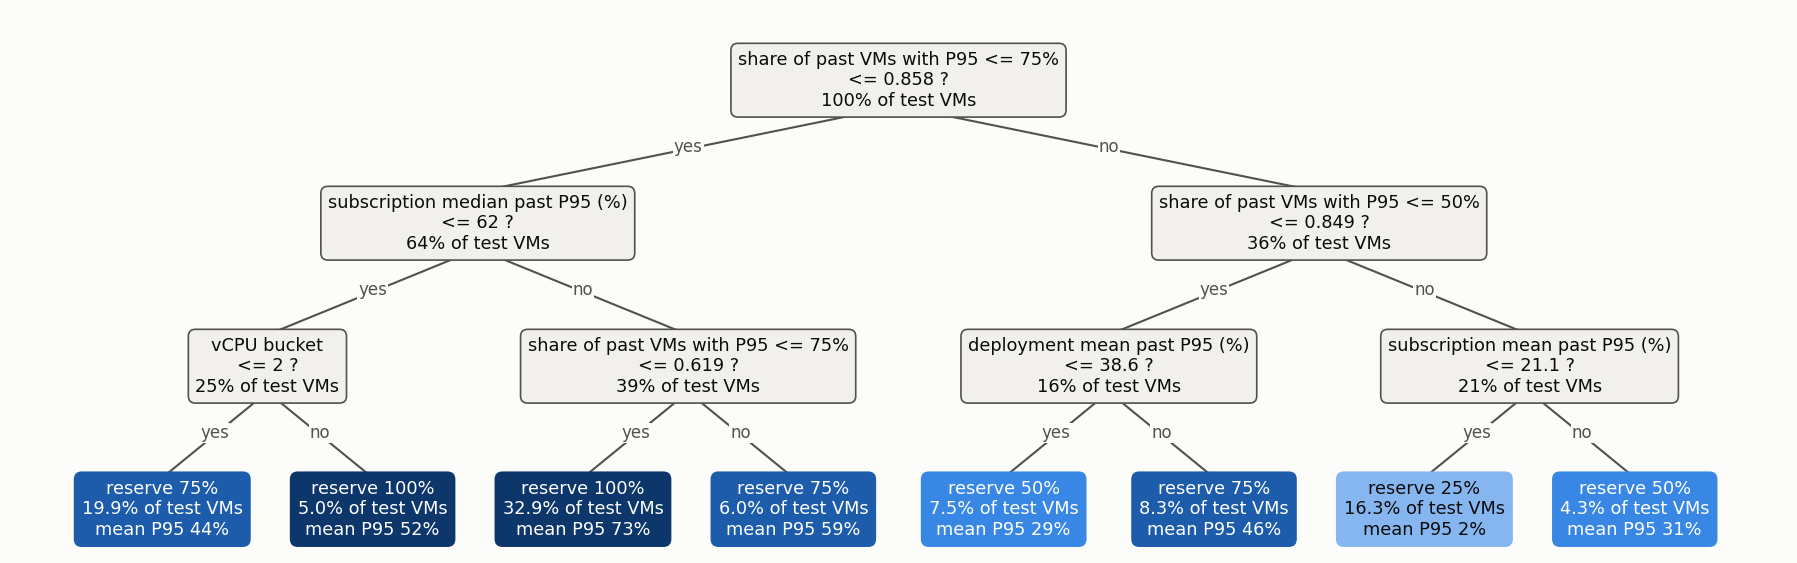
\includegraphics[width=\textwidth]{figures/fig_opt_tree.png}
\vspace{-1.2em}
\caption{Exact depth-3 OPT at $\beta=5$, trained on 1.70M VMs and certified optimal over the restricted class. Shares and mean realized P95 refer to the test window; darker leaves reserve more.}
\label{fig:tree}
\vspace{-0.6em}
\end{figure}

\paragraph{The learned policy.} The $\beta=5$ tree (Figure~\ref{fig:tree}) first asks how often the customer's past VMs exceeded 75\% P95, an upper-tail question rather than an average. Near-idle customers (16\% of test VMs, realized mean P95 2\%) receive 25\%; customers with frequent hot VMs keep 100\% unless their VMs are small; VM size matters only in that branch.

\paragraph{Information matters more than method.} In a nested feature ablation, size and creation time alone give $\beta=5$ savings of 6.0\% (OPT), 5.4\% (greedy) and 7.2\% (cost-aware RF), and at most 0.9\% at $\beta=10$. Adding subscription history raises them to 20.3\%, 20.2\% and 20.9\%; deployment history then changes little (20.1\%, 20.0\%, 21.6\%). Customer history enables personalization; the choice of method adds at most about 1.5 points.

\paragraph{Prediction accuracy versus decision quality.} The RF predicts P95 best (test $R^2$ 0.525 versus 0.494 for Ridge and 0.491 for CART), yet its root mean squared error of 25.0\pp{} equals one tier width and one VM in six is under-predicted by more than 25\pp. Rounding these unbiased predictions up under-provisions 29.9\% of VMs and is worse than the fixed rule for $\beta\ge8$. A tuned margin repairs much of this, but the three regressors with margins differ by at most 2.2 points, not in the order of their $R^2$; \S\ref{sec:refine} isolates the effect of the decision rule with the forest held fixed.

\paragraph{Exact versus greedy versus forest.} Exact optimization lowers \emph{training} cost by 0.4--0.5\% relative to the greedy tree, as it must, but the test gain is small: OPT minus greedy is $-0.0012$ [$-0.0058$, 0.0040] at $\beta=2$, $-0.0013$ [$-0.0054$, 0.0027] at $\beta=5$ and $-0.0057$ [$-0.0110$, $-0.0014$] at $\beta=10$. On an equal 200,000-VM sample greedy is slightly cheaper at $\beta=5$. One variable family, the customer's past P95 distribution, dominates, so greedy splitting rarely gets trapped. Exactness does buy stability: from 200,000 training VMs up the exact tree is identical across five samples, unlike local-search OPT. The cost-aware RF is 1.6--1.9\% cheaper than either tree, the price of interpretability here.

\paragraph{Targeting, not uniform reduction.} At $\beta=5$, OPT reserves 26.6 points less than the fixed rule and pays a shortfall penalty of 6.5 points of cost. Assigning OPT's own tier mix to VMs \emph{at random} would raise expected shortfall from 1.30\pp{} to 8.0\pp{} and cost 13.4\% \emph{more} than always reserving 100\%; a randomized fixed-tier rule with OPT's expected shortfall must reserve 93\% of capacity, against OPT's 73\% (Figure~\ref{fig:beta}b). All of the savings come from identifying which VMs can safely run on a lower tier.

\section{Refinements from the book}
\label{sec:refine}

Homework~6 Question~2(b) selected suggestion \#7, interpretable clustering with k-means and Optimal Classification Trees \citep[Ch.~20, \S\S20.1--20.2]{bertsimas2019mlopt}, and suggestion \#10, distribution-aware forest-weighted prescriptions \citep[Ch.~13, \S\S13.1--13.2]{bertsimas2019mlopt}. Both were implemented as planned on the same strict split, with every choice made on validation (Table~\ref{tab:refine}).

\begin{table}[t]
\centering\small
\caption{Refinements from the book: test cost and saving at $\beta=2,5,10$, and the $\beta=5$ operating point. Rules A--C share one P95 forest. Existing methods repeated for reference.}
\label{tab:refine}
\setlength{\tabcolsep}{3.6pt}
\begin{tabular}{lrrr|rrr|rrr}
\toprule
 & \multicolumn{3}{c|}{Test cost} & \multicolumn{3}{c|}{\% saving} & \multicolumn{3}{c}{$\beta=5$} \\
Policy & $\beta{=}2$ & $\beta{=}5$ & $\beta{=}10$ & $\beta{=}2$ & $\beta{=}5$ & $\beta{=}10$ & $\Ex[r]$ & $P(Y{>}r)$ & $\Ex[(Y{-}r)^+]$ \\
\midrule
\multicolumn{10}{l}{\emph{Refinement 1: interpretable clustering (Ch.~20)}} \\
k-means ($K=8$) $\to$ tier per cluster & 0.703 & 0.803 & 0.870 & 11.0 & 19.7 & 13.0 & 72.9 & 9.9 & 1.49 \\
OCT depth 4 $\to$ cluster $\to$ tier & 0.701 & 0.805 & 0.869 & 11.3 & 19.5 & 13.1 & 74.0 & 9.1 & 1.30 \\
\multicolumn{10}{l}{\emph{Refinement 2: distribution-aware prescription (Ch.~13), one forest}} \\
A: point prediction, rounded up & 0.697 & 0.858 & 1.125 & 11.7 & 14.2 & $-$12.5 & 59.0 & 29.9 & 5.35 \\
B: point prediction + margin & 0.692 & 0.802 & 0.847 & 12.4 & 19.8 & 15.3 & 73.2 & 10.0 & 1.41 \\
C: forest-weighted prescription & 0.685 & 0.786 & 0.835 & 13.2 & 21.4 & 16.5 & 72.5 & 9.2 & 1.22 \\
\midrule
Exact OPT, depth 3 & 0.699 & 0.799 & 0.847 & 11.5 & 20.1 & 15.3 & 73.4 & 9.3 & 1.30 \\
Cost-aware RF (separate forest) & 0.687 & 0.784 & 0.833 & 12.9 & 21.6 & 16.7 & 72.5 & 9.1 & 1.18 \\
\bottomrule
\end{tabular}
\vspace{-0.5em}
\end{table}

\subsection{Refinement 1: Interpretable clustering (Chapter 20, Sections 20.1--20.2)}

\paragraph{Implementation.} Following \S20.1 we ran k-means \citep{lloyd1982kmeans} on eight creation-time features: $\log_2$ vCPU, $\log_2$ memory, the subscription's mean and median past P95, its shares of past VMs with P95 above 75\% and above 50\%, $\log(1+\text{completed subscription VMs})$ and the deployment's mean past P95. The log transforms reduced the skewness of vCPU from 4.1 to 1.7 and of the VM count from 2.7 to $-0.5$. Features were standardized to zero mean and unit variance with a scaler fit on the strict training rows, and k-means (5 restarts, seed 0) was fit on training rows only. Among $K\in\{3,5,8,10\}$, with or without circular creation-hour features, validation cost at $\beta=5$ selected $K=8$ without hour, which also had the best silhouette (0.39 versus 0.22). Each cluster then receives the tier with the lowest \emph{training} cost for each $\beta$. The clusters are formed by feature similarity, not cost; only the tier assignment uses the cost, and no test data enters either step. Following \S20.2 and \citet{bertsimas2017oct,bertsimas2021clustering}, Optimal Classification Trees (Interpretable AI local search, minimum leaf 1,000) learn to reproduce the cluster labels from the raw, unstandardized features on a fixed 200,000-VM training sample, with depth (2--4) chosen by validation cost at $\beta=5$. A new VM follows the OCT to a predicted cluster and receives that cluster's tier.

\paragraph{Results.} The eight clusters order by the customer's past P95 level and upper-tail frequency, with VM size separating similar groups: near-idle 4-vCPU customers (15\% of VMs, realized mean P95 4\%) get 25\% at $\beta=5$, low-utilization customers 50\%, two mid-level groups 75\%, and four groups of large or hot VMs 100\%. The OCT reproduces the k-means labels on test VMs with 61.6\%, 86.1\% and 88.9\% agreement at depths 2, 3 and 4; at depth 3 it clearly beats a greedy CART classifier (74.5\%), while at depth 4 CART is slightly higher (90.8\%). Agreement barely moves cost because misassigned VMs mostly land in clusters with the same or an adjacent tier (OCT minus k-means: $+0.0015$ [$-0.0067$, 0.0105] at $\beta=5$). The cluster policy saves 19.7\% at $\beta=5$, statistically indistinguishable from OPT's 20.1\% ($+0.0044$ [$-0.0047$, 0.0140]) at a similar operating point, but falls clearly behind at $\beta=10$ (13.0\% versus 15.3\%; $+0.0228$ [0.0103, 0.0365]) and trails the cost-aware RF at every $\beta$.

\paragraph{Interpretation.} The natural workload groups in this trace already align with the tiers, which is why unsupervised segmentation recovers about 98\% of OPT's savings at $\beta=5$. The weakness at high $\beta$ follows from clustering on similarity rather than cost: at $\beta=10$ the expensive mistakes concentrate among customers with a heavy upper tail, which OPT isolates with a threshold on the share of past VMs above 75\%; the k-means boundaries do not align with it, so the cluster policy under-provisions more VMs (4.5\% versus 3.4\%). Clustering is a useful compact description of the customer population and a check on OPT, but not a substitute for optimizing the cost directly.

\subsection{Refinement 2: Distribution-aware prescriptive optimization (Chapter 13, Sections 13.1--13.2)}

\paragraph{Implementation.} Section 13.1 frames the decision as minimizing conditional expected cost, and \S13.2 estimates that expectation with weights over training observations \citep{bertsimas2020predictive}. We fit one P95 forest $\{L_t\}_{t=1}^{T}$ ($T=100$; leaf size chosen among $\{50,500,2000\}$ on validation, selecting 50, which is the main RF of \S\ref{sec:methods}). For a new VM $x$, training VM $i$ receives weight $w_i(x)$ and the prescription is
\begin{equation}
w_i(x)=\frac{1}{T}\sum_{t=1}^{T}\frac{\mathbb{1}\{x_i\in L_t(x)\}}{|L_t(x)|},\qquad
\hat r(x)\in\arg\min_{r\in\mathcal{R}}\ \sum_{i=1}^{n} w_i(x)\big[r+\beta\,(Y_i-r)^+\big],
\label{eq:forest}
\end{equation}
where $L_t(x)$ is the leaf of tree $t$ containing $x$; the weights sum to one, as in quantile regression forests \citep{meinshausen2006qrf}. Because the cost is linear in the shortfall, each leaf stores the count and three shortfall sums of its training VMs, so \eqref{eq:forest} is evaluated exactly for every $\beta$ without a dense weight matrix; tests confirm that explicit weight vectors reproduce the aggregated costs. On this \emph{same} forest we compare (A) rounding the point prediction up, (B) adding a validation-tuned margin before rounding, and (C) the prescription \eqref{eq:forest}; A and B reproduce the main pipeline's RF rules exactly. C is also compared with the cost-aware RF, OPT and the fixed rule.

\paragraph{Results.} C is cheaper than B at every $\beta$: by 0.0070 [0.0042, 0.0111] at $\beta=2$, 0.0167 [0.0117, 0.0230] at $\beta=5$ and 0.0120 [0.0015, 0.0246] at $\beta=10$ (marginal). Against A the gain is large (0.072 at $\beta=5$; 0.290 at $\beta=10$, where A is worse than the fixed rule). C beats OPT at every $\beta$ (0.0134 [0.0073, 0.0204] at $\beta=5$) and ties the cost-aware RF ($+0.0016$ [$-0.0030$, 0.0069]). At $\beta=5$, C reserves less than B (72.5\% versus 73.2\%) \emph{and} has lower expected shortfall (1.22 versus 1.41\pp) and fewer severe shortfalls (2.2\% versus 2.8\%), the last two with intervals excluding zero. At $\beta=10$ it reserves 3.2 points more than B but cuts exceedance from 5.8\% to 2.8\%.

\paragraph{Why C beats B with the same predictions.} A margin is one global shift; C adapts to the shape of each VM's conditional demand. The forest's point predictions are calibrated on average (within 3.4\pp{} of realized means in every 10-point prediction bin), but each bin is wide. Among VMs predicted at 40--50\% (24\% of test VMs), realized P95 spans 3\% to 84\% between the 10th and 90th percentiles, covering all four tiers. Rounding up reserves 50\% for all of them and leaves 41\% exceeded; C reserves 75\% on average there and leaves 16\% exceeded, while reserving 25\% for VMs whose neighbors are reliably idle. The weighted shortfall estimates are calibrated on average (expected versus realized: 0.284 vs 0.285 at 25\%, 0.145 vs 0.145 at 50\%, 0.049 vs 0.049 at 75\%). Holding the forest fixed, replacing a point estimate by its leaf-weighted distribution closes the whole gap between predict-then-decide and direct cost learning: accurately predicting expected utilization is not the same as choosing the reservation that minimizes expected cost.

\section{Sensitivity and robustness}
\label{sec:robust}

\begin{figure}[t]
\centering
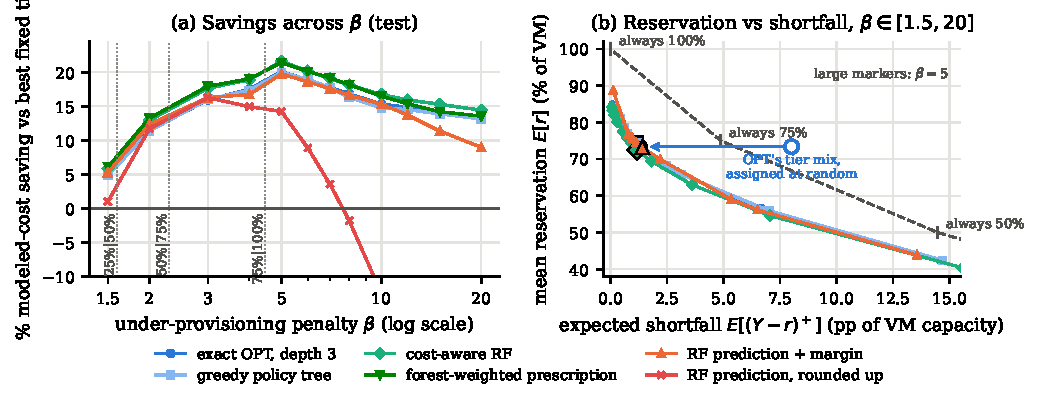
\includegraphics[width=\textwidth]{figures/fig_beta_risk.pdf}
\vspace{-1.4em}
\caption{(a) Test saving relative to the validation-selected best fixed tier at 12 values of $\beta$, with every policy re-tuned on validation at each $\beta$; dotted lines mark the validation $\beta$ at which the best fixed tier changes. (b) Mean reservation versus expected shortfall of the same configurations (lower left is better). Dashed: fixed tiers and their random mixtures. Hollow circle: OPT's $\beta=5$ tier mix assigned at random.}
\label{fig:beta}
\vspace{-0.6em}
\end{figure}

\paragraph{Economic sensitivity.} Because $\beta$ is assumed, every method was re-tuned on validation at 12 values from 1.5 to 20 (Figure~\ref{fig:beta}a); costs at different $\beta$ are never compared to choose $\beta$. OPT's saving is 5.2\% at $\beta=1.5$, 11.5\% at 2, 15.9\% at 3, 20.1\% at 5, 15.3\% at 10 and 13.3\% at 20. The peak near 5 has a simple cause: on validation the best fixed tier jumps from 75\% to 100\% at $\beta=4.46$, so just above that point the uniform baseline is most wasteful. (On test the switch is at 5.12; against a hindsight 75\% baseline OPT's $\beta=5$ saving is 19.6\%.) The method ranking is identical at all 12 values, and the cost-aware RF beats OPT at all of them. The $\beta=5$ tree tolerates a misjudged penalty: for a true $\beta$ in $[4,8]$ it costs under 1\% more on test than a tree re-optimized for the true value, rising to 2--3\% at 3 or 10 and 15--17\% at 1.5 or 20, with over-estimation the safer error.

\paragraph{Tree complexity.} Table~\ref{tab:complex} compares exact trees of different sizes. The depth-3 tree is the main, validation-selected model; the others are diagnostic variants chosen by their own validation rules (a tuned depth-2 tree; the simplest tree within 0.1\% of the best validation cost along the exact path of a per-leaf penalty; certified depth-4 solves). A four-leaf tree keeps 98.6\% of the eight-leaf savings at $\beta=5$ and 94--100\% across all 12 values of $\beta$, with no significant cost difference at $\beta=2,5,10$. Depth 4 doubles the leaves for 0.5--1.0\% lower test cost, significant only at $\beta=2$ and 10, and at $\beta=10$ it does so by reserving 1.5 points less while exceedance rises from 3.4\% to 4.6\%. Returns to depth diminish quickly; the four- and five-leaf trees are the most defensible operational rules.

\begin{table}[t]
\centering\small
\caption{Complexity and customer-level outcomes at $\beta=5$ (test). $\Delta$: paired cost difference to depth-3 OPT, 95\% subscription-clustered interval. Equal-subscription columns weight each of the 1,036 subscriptions with $\ge5$ test VMs equally (exploratory).}
\label{tab:complex}
\setlength{\tabcolsep}{4pt}
\begin{tabular}{lrrlrr|rr}
\toprule
 & & & & & & \multicolumn{2}{c}{Equal-subscription} \\
Policy & Leaves & Cost & $\Delta$ vs depth-3 OPT [95\% CI] & $\Ex[r]$ & $P(Y{>}r)$ & \% saving & $P(Y{>}r)$ \\
\midrule
Exact OPT, depth 2 & 4 & 0.802 & $+0.0028$ [$-0.0017$, 0.0079] & 74.6 & 7.7 & 18.2 & 11.2 \\
Exact OPT, leaf-penalized & 5 & 0.796 & $-0.0029$ [$-0.0101$, 0.0027] & 73.5 & 8.6 & 18.5 & 11.7 \\
\textbf{Exact OPT, depth 3} & 8 & 0.799 & -- & 73.4 & 9.3 & 17.6 & 13.1 \\
Exact OPT, depth 4 & 16 & 0.795 & $-0.0040$ [$-0.0088$, 0.0002] & 73.8 & 8.4 & 18.1 & 12.4 \\
Greedy policy tree & 5 & 0.800 & $+0.0013$ [$-0.0027$, 0.0054] & 74.3 & 8.1 & 18.3 & 11.4 \\
Cost-aware RF & -- & 0.784 & $-0.0149$ [$-0.0238$, $-0.0069$] & 72.5 & 9.1 & 18.9 & 10.3 \\
\bottomrule
\end{tabular}
\vspace{-0.5em}
\end{table}

\paragraph{Operational risk.} The objective penalizes the \emph{magnitude} of shortfall, not its frequency, so lower cost need not mean fewer exceedances. Even the oracle exceeds on 9.9\% of VMs at $\beta=5$ (24\% at $\beta=2$), because a small overshoot is cheaper than the next tier. The difference is severity: 13--14\pp{} per exceedance versus 2.5\pp{} for the oracle. The 95th percentile of shortfall given exceedance is 36.7\pp{} for OPT and 28.6\pp{} for the cost-aware RF, and about 80\% of OPT's exceedances are VMs with realized P95 above 75\%. Two-tier under-reservation is rare (0.7\% of VMs), while 19\% of VMs remain two or more tiers above need. At $\beta=5$ the cost-aware RF is at least as good as OPT on every risk measure in point estimate (none individually significant), but at $\beta=2$ its lower cost comes with 2.3 points more exceedance, a trade-off the cost objective does not reveal.

\paragraph{Customer heterogeneity.} At $\beta=5$ the median subscription (with $\ge5$ test VMs) saves 10.4\% under OPT, half the aggregate 20.1\%. The 94 subscriptions with at least 1,000 test VMs hold 78\% of test VMs and deliver 85\% of OPT's saving, though the ten largest save only 10.4\%. Under OPT, 11.9\% of subscriptions have higher modeled cost than under always-100\% (7.6--7.7\% under greedy, the four-leaf tree and the cost-aware RF), and 5.6\% lose more than 10\%. Weighting subscriptions equally (Table~\ref{tab:complex}) reverses the order of the trees: the eight-leaf OPT has the lowest saving and the highest exceedance, and greedy, the four-leaf tree and the cost-aware RF are cheaper per subscription by 0.006--0.013 with intervals excluding zero. Validation shows the same pattern (15.9\% versus 12.5--13.9\%), plausibly because the extra leaves fit a training cost dominated by large customers. This is exploratory, not a fairness objective, but VM-weighted averages can hide weaker outcomes for smaller customers.

\section{Limitations and conclusion}
\label{sec:conclusion}

\paragraph{Limitations.} All savings are modeled: $\beta$ is assumed, the tiers are hypothetical, and observed P95 stands in for demand that might change under a smaller allocation, so we claim nothing about Azure billing, throttling, consolidation or SLA compliance. The optimality certificate covers the training objective over depth-limited trees on 8 features and at most 31 thresholds per feature, not out-of-sample performance. The data cover one region and 30 days with a five-day test window; the P95 of short-lived VMs rests on few readings, and the label rule removes most long-lived training VMs, consistent with 1--5 points lower vCPU-hour-weighted savings. Features were selected once at $\beta=5$, validation selection is noisy (a smaller minimum leaf would have given OPT 0.796 instead of 0.799), and the bootstrap intervals hold policies fixed without multiplicity adjustment.

\paragraph{Conclusion.} Historical customer utilization supports interpretable reservation policies that cut modeled capacity cost by about 20\% at $\beta=5$ and 15--20\% for $\beta\in[3,10]$, with mostly mild shortfalls. The gains come from matching reservations to workloads and require learning from the cost rather than from prediction error: the same forest saves 14.2\% or 21.4\% depending only on the decision rule. Exact optimization makes OPT certifiable, fast and stable, but it barely beats greedy trees out of sample, a four-leaf tree does as well, and a cost-aware forest remains about 1.5 points cheaper. A deployment would need a shadow evaluation with enforced reservations and measured performance, a $\beta$ calibrated from service-level costs, and monitoring of customer-level outcomes alongside the aggregate.

{\footnotesize
\bibliographystyle{abbrvnat}
\bibliography{references}
}

\end{document}
